%% ----------------------------------------------------------------------------
% CVG SA/MA thesis template
%
% Created 03/08/2024 by Tobias Fischer
%% ----------------------------------------------------------------------------
\chapter{Appendix}

% -------- Instructions for writing the appendix section:
% In the appendix, list the following material: 

% \begin{itemize}
 % \item Data (evaluation tables, graphs etc.)
 % \item Program code
 % \item Further material 
% \end{itemize}

\section{Qualitative Analysis of the Current State of the Art}

As a preliminary study, we tested several state-of-the-art methods on selected human-centric scenes. This section summarizes qualitative results for representative approaches and groups them into video diffusion methods and optimization-based pipelines.

\subsection{Video Diffusion}

\begin{figure}[!ht]
    \centering
    \includegraphics[width=0.8\textwidth]{figures/appendix_video_diff_limits.drawio.png}
    \caption{\textbf{Limitations of video diffusion methods}. We show novel view synthesis results of Generative Camera Dolly \cite{vanhoorick2024gcd} (first row) and SVD4D 2.0 \cite{sv4d} (second row) on different videos.}
    \label{fig:appendix_video_diff_limits}  
\end{figure}

Figure~\ref{fig:appendix_video_diff_limits} shows qualitative results of two video diffusion methods, Generative Camera Dolly (GCD) \cite{vanhoorick2024gcd} and SVD4D 2.0 \cite{sv4d}. GCD is a conditional model that synthesizes a novel video given target camera parameters and an input monocular video. While it can produce plausible results on in-domain data such as object-centric scenes, Figure~\ref{fig:appendix_video_diff_limits} illustrates that it does not generalize reliably to human-centric scenes, where articulated motion and identity consistency are critical.


SVD4D 2.0 is a video-to-video model pretrained on a large corpus of multi-view video data. Similar to GCD, it performs well on in-domain examples, but it struggles to preserve realistic human pose and facial detail, as shown in the second row of Figure~\ref{fig:appendix_video_diff_limits}.


\subsection{Optimization-Based Methods}

\begin{figure}[!ht]
    \centering
    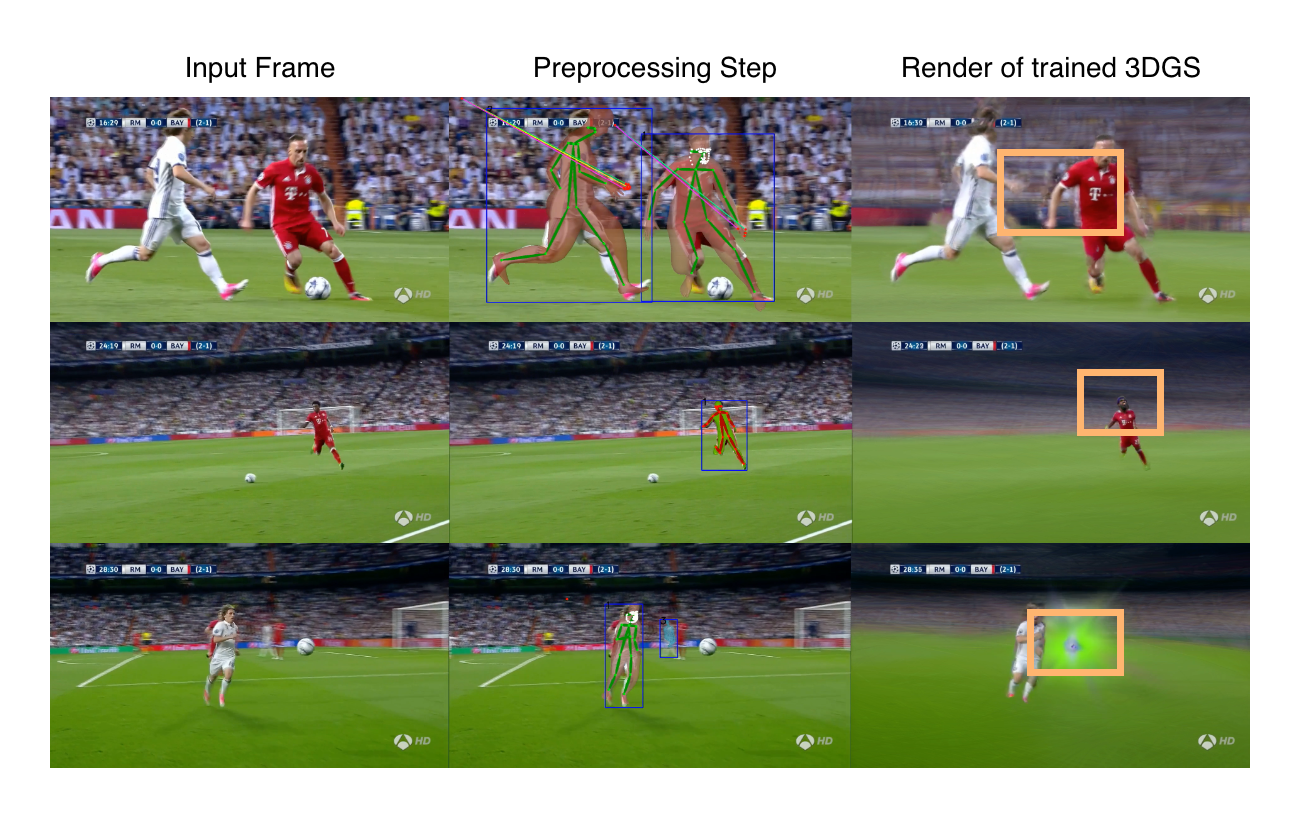
\includegraphics[width=0.8\textwidth]{figures/appendix_gtu_limits.drawio.png}
    \caption{\textbf{Limitations of the Guess the Unseen approach}. We show the input image, preprocessing outputs, and the synthesized training view produced by Guess the Unseen \cite{gtu} on different scenes.}
    \label{fig:appendix_gtu_limits}  
\end{figure}

In contrast to video diffusion methods that aim to directly synthesize a novel-view video, Guess the Unseen (GTU) \cite{gtu} is an optimization-based pipeline that reconstructs a 3D scene representation and then renders novel views from it. Figure~\ref{fig:appendix_gtu_limits} shows qualitative results of GTU on human-centric scenes. The first row highlights a failure mode where imperfect segmentation causes background appearance to leak into the dynamic human model, which leads to artifacts in the synthesized training view. The second row shows distorted facial detail, which we attribute to diffusion-based pseudo supervision producing incorrect high-frequency hallucinations. The last row shows additional artifacts around the ball that are consistent with diffusion-driven hallucinations.


\section{Instance Segmentation}
\label{sec:appendix_segmentation}

\paragraph{Metrics.}
Segmentation quality is important to accurately separate dynamic humans from the static background. We therefore measure segmentation quality using intersection-over-union (IoU), recall, and F1 score.

\subsection{Results}
\begin{figure}[!ht]
    \centering
    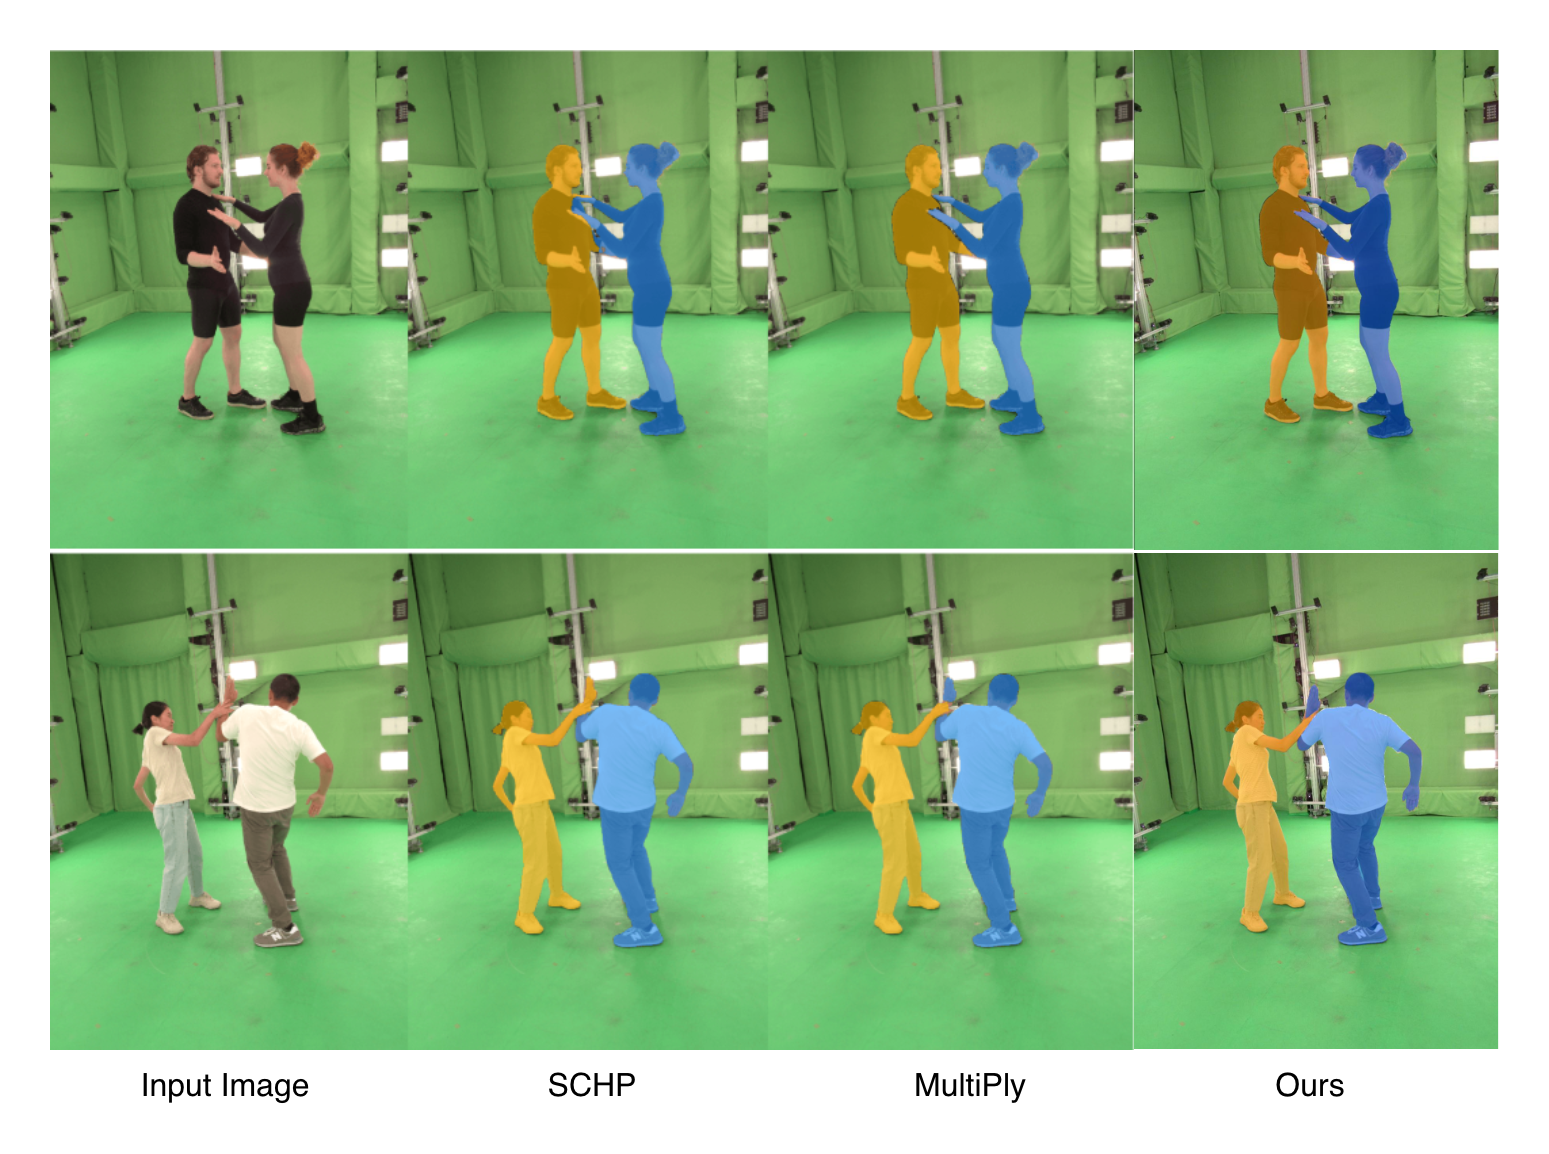
\includegraphics[width=1.0\textwidth]{figures/qual_segment_comp.drawio.png}
    \caption{\textbf{Qualitative instance segmentation comparison}. We adapt the figure from MultiPly \cite{multiply} and added our segmentation results for comparison on chosen scenes from Hi4D. For each method, we show RGB frame overlaid with predicted instance masks.}
    \label{fig:qual_instance_segm_comp}  
\end{figure}

\begin{table}[!ht]
  \centering
  \small
  \setlength{\tabcolsep}{7pt}
  \begin{tabular}{l
      S[table-format=1.3]
      S[table-format=1.3]
      S[table-format=1.3]}
    \toprule
    \textbf{Method} & \multicolumn{1}{c}{\textbf{IoU} $\uparrow$} & \multicolumn{1}{c}{\textbf{Recall} $\uparrow$} & \multicolumn{1}{c}{\textbf{F1} $\uparrow$} \\
    \midrule
    MultiPly (Init.) & 0.943 & 0.975 & 0.984 \\
    MultiPly (Progressive) & 0.963 & \textbf{0.985} & \textbf{0.990} \\
    Ours (using SAM3) & \textbf{0.974} & 0.982 & 0.987 \\
    \bottomrule
  \end{tabular}
  \caption{\textbf{Human instance segmentation results on Hi4D.} Best results are in bold.}
  \label{tab:segmentation_results_hi4d}
\end{table}

We compare our mask segmentation quality to MultiPly, which reports results for both its initial masks from SAM1 \cite{sam1} and its progressively refined masks during training. In contrast, we do not refine masks during training and rely on the initial masks from SAM3 \cite{carion2025sam3segmentconcepts}. All methods achieve strong scores, with our method obtaining the best IoU, while MultiPly's progressive masking achieves slightly higher recall and F1. This suggests different error modes: SAM3 tends to produce cleaner average overlap, while progressive refinement reduces missed foreground pixels. Overall, segmentation quality is strong and is unlikely to be the main bottleneck, although small boundary errors can still affect downstream rendering and reconstruction.

Figure \ref{fig:qual_instance_segm_comp} shows representative failure cases of our SAM3-based instance segmentation compared to MultiPly. In the top row, our method assigns part of the orange person's left arm to the blue person; in the bottom row, part of the orange person's right hand is similarly assigned to the blue person. These errors are primarily instance-level mix-ups at contact or occlusion boundaries. In practice, they are less critical for our main objective of separating dynamic humans from the static background, which both methods achieve reliably.
